% !TeX spellcheck = ru_RU
% !TEX root = vkr.tex

\section{Проектирование решения}

После полученных результатов команда \verb|TATLIN.BACKUP| провела эксперименты, где так же стало очевидно преимущество использования нескольких рантаймов с точки зрения пропускной способности.

Однако, неясным осталась надежность такой системы: разработчики \verb|tokio| не дают никаких гарантий, а наоборот утверждают, что при некотором обращении с такой конструкцией может быть наблюдаемо падение производительности или достижимо неопределенное поведение. \verb|TATLIN.BACKUP| позиционирует себя как высоконадежное производительное решение, а потому использовать в нем конструкцию без гарантий не возможно.

\subsection{Шардирование планировщика}

\begin{figure}[H]
    \begin{center}
        \makebox[\textwidth]{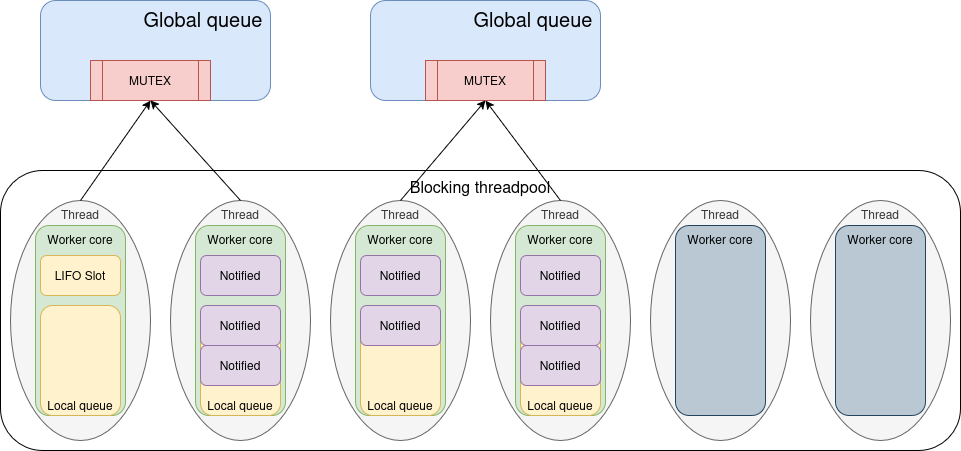
\includegraphics[scale=0.55]{pictures/tokio_duplicated.drawio.png}}
    \end{center}

    \caption{Упрощенное представление шардированного планировщика в рантайме tokio.}
    \label{fig:tokio:duplicated_arch}
\end{figure}

Если дублировать весь рантайм нельзя, вероятно, уменьшить ограничение накладываемое взаимодействием исполнителей получится при использовании нескольких изолированных  глобальных очередей и исполнителей в одном рантайме, как представлено на изображении~\ref{fig:tokio:duplicated_arch}. Здесь и далее под \verb|рабочей группой| будет пониматься глобальная очередь с фиксированным количеством исполнителей.

Такое шардирование планировщика было реализовано, так как предполагалось, что эта модификация позволит увеличить пропускную способность: каждая рабочая группа изолирована от остальных, то есть исполнители не могут похищать задачи из глобальных или локальных очередей других групп, это вынуждает их останавливать исполнение собственных потоков --- все это позволяет избежать конфликтов между исполнителями из различных групп и экономить системные ресурсы при нехватке задач.

При аллокации асинхронного замыкания ранее использовался метод \verb|tokio::spawn|. Теперь при аллокации асинхронного замыкания необходимо выбрать рабочую группу для его выполнения, для чего используется локальное для потока состояние~\cite{xorshiftRNG}. Для локализации задач акторов, созданных одной задачей производителем интерфейс был дополнен методом \verb|tokio::spawn_into()|, позволяющим пользователю сообщать желаемый номер рабочей группы для исполнения замыкания. Это позволяет пользователю распределять задачи производители между рабочими группами.

Для подтверждения гипотезы об улучшении пропускной способности с помощью шардирования планировщика необходимо произвести повторные эксперименты и сравнить использование рабочих групп с дублированием всего рантайма.
